% ============================================================================
%  VNPhish --- defence deck, DRAFT 1
%  Compile: xelatex main.tex   (twice, for the outline)
%
%  Structure follows the report, not a generic "background -> method -> results"
%  template. Slide 2 is the problem; there is no scam-history warm-up.
%
%  \pause is used throughout so each slide arrives one point at a time, the way
%  a PowerPoint build does. Nothing appears before it is being spoken about.
%
%  Every slide carries a \note{} with the report section it comes from, so an
%  answer can always be traced back to a page.
% ============================================================================
\documentclass[aspectratio=169,11pt]{beamer}
\usetheme{default}
\usefonttheme{professionalfonts}
\setbeamertemplate{navigation symbols}{}

\usepackage{fontspec}
\setmainfont{Times New Roman}
%% Central color token — change one hex value to recolor the whole deck
\definecolor{CVBLUE}{HTML}{1A5276}

%% Beamer-specific packages — only add what Beamer does NOT already load.
%% Do NOT add: fontspec, hyperref, float, caption, enumitem — all conflict or duplicate.
\usepackage{booktabs}        % table rules (\toprule, \midrule, \bottomrule)
\usepackage{colortbl}        % \cellcolor in confusion matrix
\usepackage{tikz}            % TikZ figures reused from thesis
\usetikzlibrary{calc,positioning,arrows.meta}
\usepackage{graphicx}        % \includegraphics
\usepackage{listings}        % verbatim CLI output (demo slide)
\lstset{
  basicstyle=\ttfamily\scriptsize,
  breaklines=true,
  frame=none,
  aboveskip=0pt,
  belowskip=0pt,
  columns=fullflexible,
  keepspaces=true,
}


% ---- house style -----------------------------------------------------------
\setbeamercolor{structure}{fg=CVBLUE}
\setbeamercolor{frametitle}{fg=CVBLUE}
\setbeamerfont{frametitle}{series=\bfseries,size=\large}
\setbeamerfont{framesubtitle}{size=\small}
\setbeamercolor{framesubtitle}{fg=black!55}
\setbeamertemplate{itemize item}{\color{CVBLUE}$\bullet$}
\setbeamertemplate{itemize subitem}{\color{CVBLUE!60}--}
\setbeamercolor{block title}{bg=CVBLUE!12,fg=CVBLUE}
\setbeamercolor{block body}{bg=CVBLUE!4}
\setbeamertemplate{footline}{%
  \hbox to\paperwidth{\hfill{\tiny\color{black!45}\insertframenumber}\hspace{2.2em}}\vspace{4pt}}

% a bare "fact" box used for the headline number on results slides
\newcommand{\headnum}[2]{%
  \begin{beamercolorbox}[wd=\linewidth,sep=6pt,rounded=true]{block body}%
  \centering{\Large\bfseries\color{CVBLUE}#1}\\[2pt]{\footnotesize #2}%
  \end{beamercolorbox}}

\title{Localized Vietnamese Financial Phishing Detection}
\subtitle{A local-first pipeline with explainable output}
\author{Nghiêm Xuân Sơn}
\date{October 2026}

\begin{document}

% ---------------------------------------------------------------- 1. title --
\begin{frame}[plain]
  \vfill
  \centering
  {\LARGE\bfseries\color{CVBLUE} Localized Vietnamese\\[4pt] Financial Phishing Detection\par}
  \vspace{10pt}
  {\large A local-first pipeline with explainable output\par}
  \vspace{22pt}
  {\normalsize Nghiêm Xuân Sơn \quad---\quad 23BI14388\par}
  \vspace{4pt}
  {\small University of Science and Technology of Hanoi\par}
  {\small Department of Information and Communication Technology\par}
  \vspace{14pt}
  {\footnotesize October 2026\par}
  \vfill
\end{frame}

% -------------------------------------------------------------- 2. problem --
\begin{frame}{The Problem}
  \framesubtitle{Two problems, and they pull against each other}
  \begin{itemize}\itemsep10pt
    \item Vietnamese financial phishing arrives through SMS and Zalo. The
          messages people most want checked are the ones carrying
          \textbf{bank details, phone numbers and OTP codes}.
    \pause
    \item Sending that message to a cloud service to be checked means
          \textbf{uploading exactly what needs protecting}.
    \pause
    \item A general multilingual model does not cover how these messages are
          really written: mixed Vietnamese and English, chat abbreviations,
          missing diacritics, emoji.
  \end{itemize}
  \pause
  \vfill
  \begin{block}{What this thesis builds}
    A detector that runs \textbf{on the user's own laptop}, classifies the
    message, and \textbf{shows the phrases it reacted to} instead of a bare
    confidence score.
  \end{block}
  \note{Report Sections 1.1--1.2. Do not open with scam statistics; open with
        the conflict between checking a message and protecting it.}
\end{frame}

% ------------------------------------------------------------ 3. why local --
\begin{frame}{Why It Has to Run Locally}
  \framesubtitle{The privacy argument, using the provider's own documentation}
  \begin{itemize}\itemsep8pt
    \item OpenAI's \textbf{Temporary Chat} keeps a conversation out of history,
          does not train on it, and writes no memory.
    \pause
    \item It does not stop the message being sent. OpenAI's documentation states
          a copy may be kept \textbf{up to 30 days} for safety purposes.
    \pause
    \item So under the strongest privacy setting offered, a message containing a
          bank account number and an OTP still leaves the device and sits on
          someone else's server for up to a month.
    \pause
    \item The 2023 caching bug makes the same point from the other side: that
          exposure came from \textbf{the provider's code}, not a user setting.
  \end{itemize}
  \pause
  \vfill
  \begin{block}{}
    A privacy setting is only as good as the system enforcing it. Running the
    model on the device removes the question instead of answering it.
  \end{block}
  \note{Report Section 1.9. If asked "why not just use ChatGPT privacy mode",
        this is the slide --- quote their own FAQ, do not argue.}
\end{frame}

% ------------------------------------------------------------- 4. the build --
\begin{frame}{What Was Built}
  \framesubtitle{Offline preparation, done once --- then one runtime path per message}
  \centering
  % the thesis figure is drawn for a 14.6 cm page; a 16:9 slide is narrower
  \resizebox{\linewidth}{!}{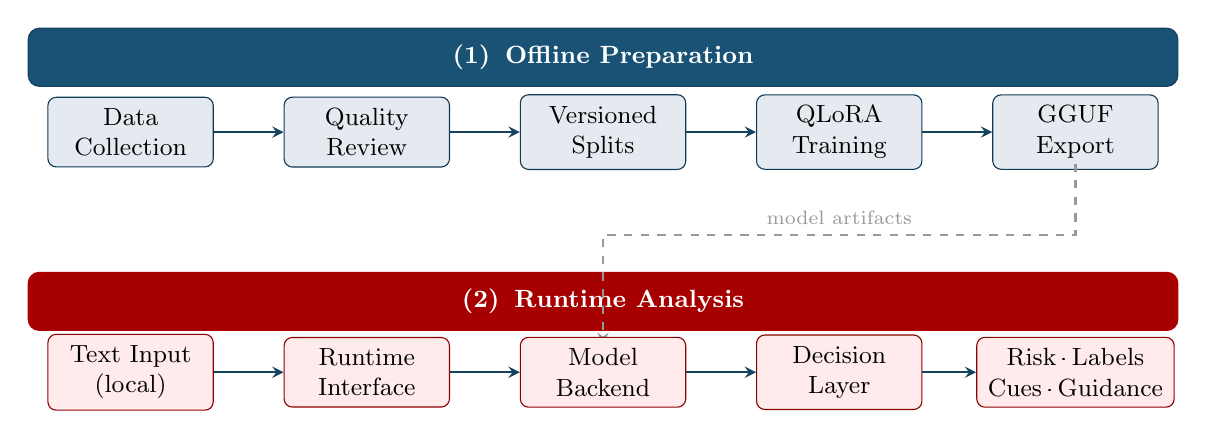
\begin{tikzpicture}[
  %% Offline-row boxes — light CVBLUE fill
  obox/.style={
    draw=CVBLUE!70!black, fill=CVBLUE!12, rectangle, rounded corners=3pt,
    minimum width=2.1cm, minimum height=0.80cm,
    align=center, font=\small, inner sep=4pt
  },
  %% Runtime-row boxes — light crimson fill
  rbox/.style={
    draw=red!55!black, fill=red!8, rectangle, rounded corners=3pt,
    minimum width=2.1cm, minimum height=0.80cm,
    align=center, font=\small, inner sep=4pt
  },
  %% Section header bars — solid CVBLUE / crimson
  ohdr/.style={
    draw=CVBLUE!80!black, fill=CVBLUE, rectangle, rounded corners=4pt,
    minimum width=14.6cm, minimum height=0.52cm,
    align=left, font=\small\bfseries, text=white, inner sep=6pt
  },
  rhdr/.style={
    draw=red!70!black, fill=red!65!black, rectangle, rounded corners=4pt,
    minimum width=14.6cm, minimum height=0.52cm,
    align=left, font=\small\bfseries, text=white, inner sep=6pt
  },
  arr/.style={->, >=stealth, thick, CVBLUE!80!black},
  darr/.style={->, >=stealth, thick, dashed, black!40}
]

%% ── Headers ──────────────────────────────────────────────────
\node[ohdr] at (0,  0.00) {(1)\enspace Offline Preparation};
\node[rhdr] at (0, -3.10) {(2)\enspace Runtime Analysis};

%% ── Offline row  (3 cm spacing → 0.9 cm gap) ─────────────────
\node[obox] (dc)  at (-6.0, -0.95) {Data\\Collection};
\node[obox] (qrv) at (-3.0, -0.95) {Quality\\Review};
\node[obox] (spl) at ( 0.0, -0.95) {Versioned\\Splits};
\node[obox] (qlo) at ( 3.0, -0.95) {QLoRA\\Training};
\node[obox] (gex) at ( 6.0, -0.95) {GGUF\\Export};

\draw[arr] (dc)  -- (qrv);
\draw[arr] (qrv) -- (spl);
\draw[arr] (spl) -- (qlo);
\draw[arr] (qlo) -- (gex);

%% ── Handoff arrow ────────────────────────────────────────────
\draw[darr]
  (6.0, -1.35) -- (6.0, -2.26)
  -- node[above, font=\scriptsize, text=black!40] {model artifacts}
  (0.0, -2.26)
  -- (0.0, -3.64);

%% ── Runtime row ──────────────────────────────────────────────
\node[rbox] (inp) at (-6.0, -4.00) {Text Input\\(local)};
\node[rbox] (rif) at (-3.0, -4.00) {Runtime\\Interface};
\node[rbox] (mod) at ( 0.0, -4.00) {Model\\Backend};
\node[rbox] (dly) at ( 3.0, -4.00) {Decision\\Layer};
\node[rbox, minimum width=2.25cm] (out) at ( 6.0, -4.00)
  {Risk\,·\,Labels\\Cues\,·\,Guidance};

\draw[arr] (inp) -- (rif);
\draw[arr] (rif) -- (mod);
\draw[arr] (mod) -- (dly);
\draw[arr] (dly) -- (out);

\end{tikzpicture}
}
  \pause
  \vfill
  \begin{block}{}
    \small The only thing crossing between the two halves is the trained model
    file. At runtime nothing needs an API key or an internet connection.
  \end{block}
  \note{Report Figure 3.1. Say: top row happens once, bottom row happens every
        time a user checks a message.}
\end{frame}

% ------------------------------------------------------------ 5. objectives --
\begin{frame}{Objectives, and What Was Actually Met}
  \begin{columns}[T,onlytextwidth]
    \begin{column}{0.52\textwidth}
      {\small\textbf{Seven objectives}}
      \begin{enumerate}\small\itemsep2pt
        \item Build a Vietnamese phishing dataset
        \item Review part of it by hand
        \item Repair what came out badly
        \item Choose the base model by measuring
        \item Check that fine-tuning was needed
        \item Measure LoRA against QLoRA
        \item Train, export, evaluate once
      \end{enumerate}
    \end{column}
    \pause
    \begin{column}{0.44\textwidth}
      {\small\textbf{Not finished}}\\[4pt]
      {\small
      \begin{itemize}\itemsep4pt
        \item No deployment version fitted after the evaluation --- on purpose,
              a single final evaluation loses its meaning if training continues
              on the same data.
        \item The code was reorganised, but a later review left security
              findings open.
      \end{itemize}}
    \end{column}
  \end{columns}
  \note{Report Chapter II. Volunteering the two unfinished items here is
        cheaper than being asked about them later.}
\end{frame}

% ---------------------------------------------------------------- 6. data --
\begin{frame}{The Dataset}
  \framesubtitle{2,097 Vietnamese messages, four classes}
  \begin{columns}[T,onlytextwidth]
    \begin{column}{0.5\textwidth}
      {\small
      \begin{itemize}\itemsep6pt
        \item Written from \textbf{public scam-warning articles} on
              \textit{tinnhiemmang.vn}, not collected from victims.
        \pause
        \item 1,658 train / 219 validation / \textbf{220 set aside}.
        \pause
        \item Every message stores the ID of the article it came from.
      \end{itemize}}
    \end{column}
    \pause
    \begin{column}{0.46\textwidth}
      \begin{block}{The rule that matters}
        \small All messages from one article go into the \textbf{same} part.
        Two messages from one article can differ by a bank name and an amount,
        so splitting them would test the model on near-copies of its own
        training data.
      \end{block}
    \end{column}
  \end{columns}
  \pause
  \vfill
  {\footnotesize In the training messages: \textbf{31.4\%} carry chat
  abbreviations, \textbf{12.9\%} are typed with no diacritics, \textbf{6.3\%}
  contain emoji.}
  \note{Report Sections 1.1 and 3.2. The 8\% cap on any single article held at
        7.9638\%.}
\end{frame}

% ------------------------------------------------------------ 7. quality ----
\begin{frame}{Data Quality --- The Uncomfortable Part}
  \framesubtitle{Reported as measured, not as hoped}
  \begin{itemize}\itemsep7pt
    \item A judge model scored every message. \textbf{1,395 of 2,097 passed
          (66.52\%)} --- a message fails if any one of five checks scores below
          3 out of 5.
    \pause
    \item A Vietnamese-speaking reviewer checked 100 by hand: \textbf{44
          passed}, and the reviewer agreed with the judge on 87 of 100.
    \pause
    \item Of 324 doubtful labels reviewed, 233 corrections were agreed but
          \textbf{only 57 were used} --- the other 176 all came from one
          article, and admitting them would inflate a class with near-copies.
  \end{itemize}
  \pause
  \vfill
  \begin{block}{The limitation to say out loud}
    \small The rewritten Zalo messages pass at 99.7\%, task scam at 47.5\%.
    That gap is not quality --- the Zalo messages were rewritten by a model from
    the \textbf{same family as the judge}. For those, the judge is not an
    independent opinion.
  \end{block}
  \note{Report Section 5.2. Say the 99.7\% caveat BEFORE anyone asks about it.}
\end{frame}

% ---------------------------------------------------- 8. was tuning needed --
\begin{frame}{Was Fine-Tuning Even Necessary?}
  \framesubtitle{Measured, not assumed --- same model, same 254 messages}
  \centering
  \pause
  \headnum{macro F1 \; 0.6702 \;$\rightarrow$\; 0.9625}{prompting alone, then the same model after QLoRA}
  \pause
  \vfill
  \begin{columns}[T,onlytextwidth]
    \begin{column}{0.48\textwidth}
      {\small\textbf{What the base model actually did}}\\[4pt]
      {\small It labelled \textbf{111 of 254} messages as bank impersonation
      when only 56 were, and accepted only \textbf{21 of 61} safe messages as
      safe.}
    \end{column}
    \pause
    \begin{column}{0.48\textwidth}
      \begin{block}{}
        \small It was not detecting scams. It was calling almost everything a
        scam --- which is why the biggest gain from fine-tuning lands on the
        \textbf{benign} class.
      \end{block}
    \end{column}
  \end{columns}
  \note{Report Section 3.4.1. This is the answer to "why not just prompt a big
        model". It is our own measurement, not a citation.}
\end{frame}

% ------------------------------------------------------------ 9. hardware ---
\begin{frame}{Choosing the Training Method on Real Hardware}
  \framesubtitle{RTX 5050 laptop, 8,151 MiB --- both methods measured before committing}
  \begin{columns}[T,onlytextwidth]
    \begin{column}{0.48\textwidth}
      {\small\textbf{Ordinary LoRA}}
      \begin{itemize}\small\itemsep3pt
        \item 7,902 of 8,151 MiB used
        \item \textbf{9 MiB free} at its tightest
        \item pointed at $\sim$18 hours
        \item no out-of-memory error
      \end{itemize}
    \end{column}
    \pause
    \begin{column}{0.48\textwidth}
      {\small\textbf{NF4 QLoRA}}
      \begin{itemize}\small\itemsep3pt
        \item 7,516 of 8,151 MiB used
        \item workable margin throughout
        \item 3.46 s median per step
        \item no out-of-memory error
      \end{itemize}
    \end{column}
  \end{columns}
  \pause
  \vfill
  \begin{block}{The decision, stated honestly}
    \small LoRA \textbf{did not crash}. An eighteen-hour run with 9 MiB to spare
    is a bad bet: one brief extra allocation ends it and costs most of a day.
    The choice was about memory and risk, not about accepting a worse model.
  \end{block}
  \note{Report Sections 3.4.2 and 4.3. Never say LoRA ran out of memory. It did
        not, and the report says so.}
\end{frame}

% ----------------------------------------------------------- 10. training ---
\begin{frame}{Training the Two Models}
  \begin{columns}[T,onlytextwidth]
    \begin{column}{0.48\textwidth}
      {\small\textbf{Qwen3-4B-Instruct-2507}}
      \begin{itemize}\small\itemsep3pt
        \item NF4 QLoRA, 3 epochs, seed 42
        \item 1,245 optimizer steps
        \item checkpoint \textbf{200} selected
        \item exported to Q8\_0 GGUF, 4.28 GB
      \end{itemize}
    \end{column}
    \pause
    \begin{column}{0.48\textwidth}
      {\small\textbf{PhoBERT}}
      \begin{itemize}\small\itemsep3pt
        \item full classifier, nothing quantized
        \item 312 optimizer steps
        \item checkpoint \textbf{100} selected
        \item comparison baseline, not shipped
      \end{itemize}
    \end{column}
  \end{columns}
  \pause
  \vfill
  \begin{block}{The 14.87-hour run --- where the time actually went}
    \small The 1,245 optimizer steps account for only \textbf{1.36 hours}. The
    rest is validation: at each of 25 checkpoints the model writes a full
    structured answer for all 219 validation messages --- 5,475 generated
    answers on a laptop GPU.
  \end{block}
  \note{Report Sections 4.4--4.5. The time breakdown pre-empts the sharpest
        arithmetic question available.}
\end{frame}

% --------------------------------------------------------------- 11. demo ---
\begin{frame}{The Analysis --- Three Real Inputs}
  \framesubtitle{Run through the exported model}
  {\small
  \textbf{Input 1 --- a scam.} \textit{``{[}VIETCOMBANK{]} Tai khoan cua ban vua
  bi truy cap\ldots bam vao link de khoa ngay:
  \texttt{vcb-secure-alert.net}\ldots''}}
  \pause
  \vspace{2pt}
  {\small $\rightarrow$ \textbf{high-risk}, \texttt{bank\_impersonation}. Quoted
  the link, the 03:47 access claim, the phone number. \textbf{Correct.}}
  \pause
  \vspace{6pt}

  {\small\textbf{Input 2 --- a real transaction notice.} \textit{``VCB: TK
  0123456789 -250,000 VND\ldots THANH TOAN HOA DON DIEN EVN HANOI\ldots''}}
  \pause
  \vspace{2pt}
  {\small $\rightarrow$ \textbf{benign}. Mentions a bank, an account number and
  an amount, and is still not flagged. \textbf{Correct.}}
  \pause
  \vspace{6pt}

  {\small\textbf{Input 3 --- a real OTP notice.} \textit{``VPBank Smart OTP: Mã
  xác thực\ldots để xác nhận đăng nhập Internet Banking\ldots''}}
  \pause
  \vspace{2pt}
  {\small $\rightarrow$ \textbf{suspicious}. \textcolor{red!60!black}{Wrong ---
  this is a false alarm.}}
  \note{Report Section 4.7. Show the advice text on the next slide, not here.}
\end{frame}

% ------------------------------------------------------- 12. the false alarm --
\begin{frame}{The False Alarm --- and Why It Is Reported}
  \framesubtitle{Six ordinary bank messages tested; four returned benign}
  \begin{itemize}\itemsep8pt
    \item The two that were flagged are the \textbf{only two that ask the reader
          to log in}. All six mention a bank.
    \pause
    \item Nearly every scam in the training data works by getting someone to log
          in or hand over a code, so the model has learned to treat
          \textbf{authentication language as the signal itself}.
    \pause
    \item The mistake is in the \textbf{safer direction}: a false alarm costs a
          minute, a scam called safe can cost someone their savings.
    \pause
    \item Even with the label wrong, the advice was still safe --- check the
          official app, share the code with nobody, call the bank yourself.
  \end{itemize}
  \pause
  \vfill
  \begin{block}{}
    \small A wrong label attached to harmful advice would be a real defect. A
    wrong label attached to safe advice is a much smaller one.
  \end{block}
  \note{Report Section 4.7 and Chapter V limits. This slide is the strongest one
        in the deck: the weakness was found, named, and explained by us.}
\end{frame}

% ------------------------------------------------------------ 13. results ---
\begin{frame}{Results}
  \framesubtitle{220 messages set aside before training, seen once, at the end}
  \centering
  \pause
  \begin{table}\small
  \begin{tabular}{lccc}
    \toprule
    & \textbf{Macro F1} & \textbf{Unreadable} & \textbf{Risky called safe} \\
    \midrule
    Qwen QLoRA & 0.980493 & 0 & \textbf{1} \\
    PhoBERT    & 0.990892 & 0 & \textbf{1} \\
    \bottomrule
  \end{tabular}
  \end{table}
  \pause
  \vfill
  \begin{block}{The column that matters}
    \small A dangerous message called safe is the expensive mistake. Both models
    made \textbf{exactly one}. On the measure that matters most for a phishing
    tool, \textbf{they tied.}
  \end{block}
  \pause
  \vspace{4pt}
  {\footnotesize Each model was trained once, so the overall gap describes this
  run. It is not enough to conclude PhoBERT classifies better in general --- and
  PhoBERT cannot produce the risk tier, the evidence, or the explanation.}
  \note{Report Chapter V. Never claim significance, a stable winner, or
        run-to-run variance. One seed, one run.}
\end{frame}

% -------------------------------------------------------- 14. limitations ---
\begin{frame}{Limitations}
  \framesubtitle{Stated in the report, not discovered in this room}
  \begin{itemize}\small\itemsep6pt
    \item \textbf{The messages are generated}, written from public warnings
          rather than collected from real victims.
    \pause
    \item \textbf{Everything ran once}, one seed. No repeat run, so no statement
          about how much the numbers would move.
    \pause
    \item \textbf{The judge is not fully independent} for the rewritten Zalo
          class.
    \pause
    \item \textbf{Genuine messages that mention logging in are over-flagged},
          systematically.
    \pause
    \item \textbf{Manual checking covers a sample}, not the whole set.
    \pause
    \item \textbf{Text only.} No screenshots, no QR codes, and never tested
          against real messages arriving on a real phone.
  \end{itemize}
  \note{Report Section 5.5. Reading these aloud is cheaper than being walked
        into any one of them.}
\end{frame}

% ------------------------------------------------- 15. contributions/future --
\begin{frame}{Contributions and What Comes Next}
  \begin{columns}[T,onlytextwidth]
    \begin{column}{0.48\textwidth}
      {\small\textbf{Contributions}}
      \begin{itemize}\small\itemsep4pt
        \item A 2,097-message Vietnamese dataset with threat labels and marked
              evidence, split so near-copies cannot leak
        \item Faults found and repaired before training, with the decisions
              recorded
        \item Two models trained on one laptop; a 4.28 GB file that runs offline
        \item One evaluation, run once
      \end{itemize}
    \end{column}
    \pause
    \begin{column}{0.48\textwidth}
      {\small\textbf{Future work}}
      \begin{itemize}\small\itemsep4pt
        \item Review the whole dataset by hand, not a sample
        \item \textbf{Use both models}: PhoBERT for the label, Qwen for the
              explanation
        \item Try \textbf{ViSoBERT}, trained on Vietnamese social-media text,
              in PhoBERT's place
        \item OCR, so the user never has to open the suspicious message to copy
              its text
      \end{itemize}
    \end{column}
  \end{columns}
  \note{Report Chapter VI. The OCR point has a safety reason, not just
        convenience: copying text means opening the message next to a live link.}
\end{frame}

% ------------------------------------------------------------- 16. closing --
\begin{frame}[plain]
  \vfill\centering
  {\LARGE\bfseries\color{CVBLUE} Thank you\par}
  \vspace{12pt}
  {\normalsize Questions\par}
  \vfill
\end{frame}

% ============================== BACKUP =====================================
\appendix
\begin{frame}[plain]\centering\vfill
  {\large\bfseries\color{CVBLUE} Backup slides\par}\vfill
\end{frame}

\begin{frame}{Backup --- How the Evidence Is Grounded}
  {\small Every phrase the model claims to have found is checked against the
  message before the user sees it:}
  \vspace{4pt}
  \begin{lstlisting}
def cue_span_is_grounded(normalized_text: str, span: str) -> bool:
    normalized_span = span.strip()
    return bool(normalized_span) and \
           normalized_span.casefold() in normalized_text.casefold()
  \end{lstlisting}
  \vspace{2pt}
  {\small If the phrase does not literally appear in the message, it is dropped
  rather than displayed. \texttt{local\_model.py:597}.}
  \note{The answer to "how do you know the model is not inventing its
        evidence". Four lines of code, not an assurance.}
\end{frame}

\begin{frame}{Backup --- The Three Prompts}
  {\small Three prompts decide everything the system produces. All are quoted in
  full in Appendix 6 of the report.}
  \vspace{6pt}
  \begin{itemize}\small\itemsep6pt
    \item \textbf{Generation} --- names the target class, so the label exists
          without a person assigning it; asks for teencode and code-switching by
          name; forbids deriving the risk tier from the label.
    \item \textbf{Judging} --- five scores, pass only if all five reach 3. The
          pass rule is inside the prompt, which is why one weak score fails a
          whole message.
    \item \textbf{Runtime} --- fixes the JSON shape and carries the safety rule
          on recommendations.
  \end{itemize}
\end{frame}

\begin{frame}{Backup --- Dataset Repair, Before and After}
  {\small A Zalo message that was written as \textit{narration} rather than as a
  message:}
  \begin{block}{}
    \scriptsize\itshape ``Tin nhắn thoại trên Zalo được chép lại: `Con trai của
    \textbf{người nhận} vừa được đưa vào khoa cấp cứu. \textbf{Người gửi} nói
    cuộc gọi video\ldots'\,''
  \end{block}
  \pause
  {\small The replacement, from the same source article and the same seed:}
  \begin{block}{}
    \scriptsize\itshape ``\textbf{Tôi} vừa trao đổi nhanh qua video về tình
    trạng của cháu nhưng đường truyền trong viện bị ngắt\ldots \textbf{anh/chị}
    quét mã QR này để chuyển khoản viện phí\ldots''
  \end{block}
  {\footnotesize Judge scored the first one realism 2/5; the reviewer marked it
  FAIL. Same scenario root, rewritten in the first person, applied offline.}
\end{frame}

\end{document}
